\documentclass{article}

\usepackage{graphicx}
\usepackage{amsfonts}
\usepackage{amsmath}
\usepackage{subcaption}
\usepackage{multirow}
\usepackage{algorithm}
\usepackage{algpseudocode}
\DeclareMathOperator*{\argmax}{arg\,max}
\usepackage{corl_2023} % Use this for the initial submission.
%\usepackage[final]{corl_2023} % Uncomment for the camera-ready ``final'' version.
%\usepackage[preprint]{corl_2023} % Uncomment for pre-prints (e.g., arxiv); This is like ``final'', but will remove the CORL footnote.

\title{Formatting Instructions for CoRL 2023}

% The \author macro works with any number of authors. There are two
% commands used to separate the names and addresses of multiple
% authors: \And and \AND.
%
% Using \And between authors leaves it to LaTeX to determine where to
% break the lines. Using \AND forces a line break at that point. So,
% if LaTeX puts 3 of 4 authors names on the first line, and the last
% on the second line, try using \AND instead of \And before the third
% author name.

% NOTE: authors will be visible only in the camera-ready and preprint versions (i.e., when using the option 'final' or 'preprint'). 
% 	For the initial submission the authors will be anonymized.

\author{
  Kartik Nagpal\\
  Department of Aerospace Engineering\\
  University of Illinois Urbana-Champaign\\
  \texttt{nagpal4@illinois.edu} \\
  \And
  Negar Mehr \\
  Department of Aerospace Engineering\\
  University of Illinois Urbana-Champaign\\
  \texttt{negar@illinois.edu} \\
  %% \AND
  %% Coauthor \\
  %% Affiliation \\
  %% Address \\
  %% \texttt{email} \\
  %% \And
  %% Coauthor \\
  %% Affiliation \\
  %% Address \\
  %% \texttt{email} \\
  %% \And
  %% Coauthor \\
  %% Affiliation \\
  %% Address \\
  %% \texttt{email} \\
}


\begin{document}
\maketitle

%===============================================================================

\begin{abstract}
    The purpose of this document is to provide both the basic paper template and submission guidelines. Abstracts should be a single paragraph, between 4--6 sentences long, ideally. Gross violations will trigger corrections at the camera-ready phase.
\end{abstract}

% Two or three meaningful keywords should be added here
\keywords{CoRL, Robots, Learning} 

%===============================================================================

\section{Introduction}
	
    Submission to CoRL 2023 will be entirely electronic, via a web site (not email). Information about the submission process and \LaTeX{} templates are available on the conference web site at \url{https://corl2023.org/}. For camera ready submission, use the \texttt{final} option for the \texttt{\textbackslash usepackage} command. 

%===============================================================================


\section{Outline}
\begin{itemize}
 \item Abstract
 \item Introduction
 \begin{itemize}
     \item Define Problem
     \item Discuss Challenges
     \item Literature Review
 \end{itemize}
 \item Background: Section on Explaining MDPs and history of the assembly task (Rest of Literature Review)
 \begin{itemize}
     \item Assembly Planning, previous works
     \item Explaining MDPs
     \item Q-Learning and DQNs
     \item Graph Exploration methods?
 \end{itemize}
 \item Model Overview (Formalism, Method)
 \begin{itemize}
     \item Graph and Tree Architecture
     \item Dynamics Decoupling
     \item Constraints Definitions
     \item Exploration Algorithms
     \item DQN Architecture
 \end{itemize}
 \item Results
 \item Conclusion
\end{itemize}

Additional Ideas: 
\begin{itemize}
 \item $P(s'|s,a)$ can be used to encode chance of failure and cost of entering the failure state will can be a parameter that the user can tune to their accepted level of risk!
 \item Running example can be the 4-piece assembly seen in figure 1 and 2!
 \item specify \emph{Reinforcement Learning (RL)}
 \item edge removal is isomorphic to ordering
\end{itemize}




\color{red} 
\section{Scratchpad (Going to move correct sections later)}
\color{black}
Notation abusing deterministic policies:
\begin{equation}
    \begin{aligned}
        \max_{\tau_s, \tau_a} \quad & \sum_{s\in \tau_s, a \in \tau_a}{R(s,a)}\\
        \textrm{s.t.} \quad & P(\tau_{s}^{t+1}|\tau_s^t,\tau_a^t) = 1\\
        \textrm{s.t.} \quad & \tau_s^0 = s^0
    \end{aligned}    
\end{equation}

We formulate the assembly sequencing problem as a sequential decision-making problem as a Markov Decision Process (MDP) defined by the tuple $\left\langle s_0, \mathcal{S}, \mathcal{A}, \mathcal{T}, \mathcal{R}, \gamma\right\rangle$, where $s_0$ is the deterministic initial state, $\mathcal{S}$ and $\mathcal{A}$ are state and action spaces respectively, $\mathcal{P}: \mathcal{S} \times \mathcal{A} \rightarrow \mathcal{S}$ is the probability transition function, $\mathcal{R}: \mathcal{S} \times \mathcal{A} \times \mathcal{S} \rightarrow \mathbb{R}$ gives the reward for a given transition. The agent acts with a stochastic policy $\pi: \mathcal{S} \rightarrow \Delta_{\mathcal{A}}$, generating a sequence of state-action-reward transitions or trajectory $\tau:=\left(s_k, a_k, r_k\right)_{k \geq 0}$ with probability $p_\pi(\tau)$ and corresponding return $R(\tau):=\sum_{k \geq 0}  r_k$. The standard objective in RL is to find a return-maximizing policy that satisfies \ref{eq:optimal_pi}.
\begin{equation} \label{eq:optimal_pi}
    \pi^* = \argmax_{\pi} \mathbb{E}_{\pi, \tau}\left [\sum_{t=1}^{\tau} R(s_t,a_t) \bigg| 
    \begin{array}{c}
        s_0\\
        s_{t+1}\sim P(s_{t+1} | s_t, a_t)\\
        a_t\sim \pi(s_t)
    \end{array}
    \right ]
\end{equation}

\color{red}[Cover basics of Dynamic Programming with no discount factor]\color{black}

\begin{equation}
    \begin{aligned}
    & V^\pi\left(s_t\right)=\mathbb{E}_\pi\left[\sum_{k=t}^T \left(s_t, a_t\right) \mid s=s_t\right] \\
    & Q^\pi\left(s_t, a_t\right)=\mathbb{E}_\pi\left[\sum_{k=t}^T \left(s_t, a_t\right) \mid s=s_t, a=a_t\right] \\
    & A^\pi\left(s_t, a_t\right)=Q^\pi\left(s_t, a_t\right)-V^\pi\left(s_t\right)
    \end{aligned}
\end{equation}


\section{Background}

Assembly sequencing is the process of determining the order in which parts should be assembled to create a product. This problem is made challenging by the many factors that need consideration, from the compatibility of parts, to the availability of tools and resources at certain points in the assembly process, to constraints made on intermediary assemblies.

Traditionally, assembly sequencing problems have been solved using heuristic methods which typically exploit a characteristic of the cost structure of the problem and are effectively based on rules of thumb or experience, and they may not always produce optimal solutions.

We propose an alternative approach that rests on using graph exploration methods to solve assembly sequencing problems with arbitrary cost structures. For context, Graph exploration methods are a type of search algorithm that can be used to explore the space of possible assembly sequences. These methods are typically more efficient than heuristic methods, and they can often produce optimal solutions.

\section{Model Overview}
\color{red} [Transition sentence] \color{black} The primary insight is a smart reformulation of the assembly problem as a graph exploration task. To achieve this, the assembled structure is first posed as a connected graph structure, $\mathbf{G}$, where different nodes of the graph correspond with different parts in the assembly, and the edges between these nodes correspond to connections required to connect these parts together.

\subsection{Graph Architectures}
Intuitively, this assembled graph represents a state, and as connections are removed, additional states of the system are generated. As such, a disassembly task can be seen as an ordering of removing these edges in the graph $\mathbf{G}$, and reversing this ordering would provide an assembly strategy. If an \textit{action} is defined as removal of a connection in the $\mathbf{G}$ graph, the disassembly process becomes a series of State-Action pairs. Here the State space $\mathbf{S}$
includes all possible sub-assemblies of the structure, and the Action space $\mathbf{A}$ is simply all connections that exist in the fully assembled state.

As seen in Fig.~\ref{fig: treeGen}, this allows the construction of a tree directed graph $\mathbf{H}$ with the root being the fully assembled structure, the edges corresponding to the removal of certain connections, and the leaves corresponding to states where the structure is fully disassembled.

\begin{figure}[!htb]
\centering
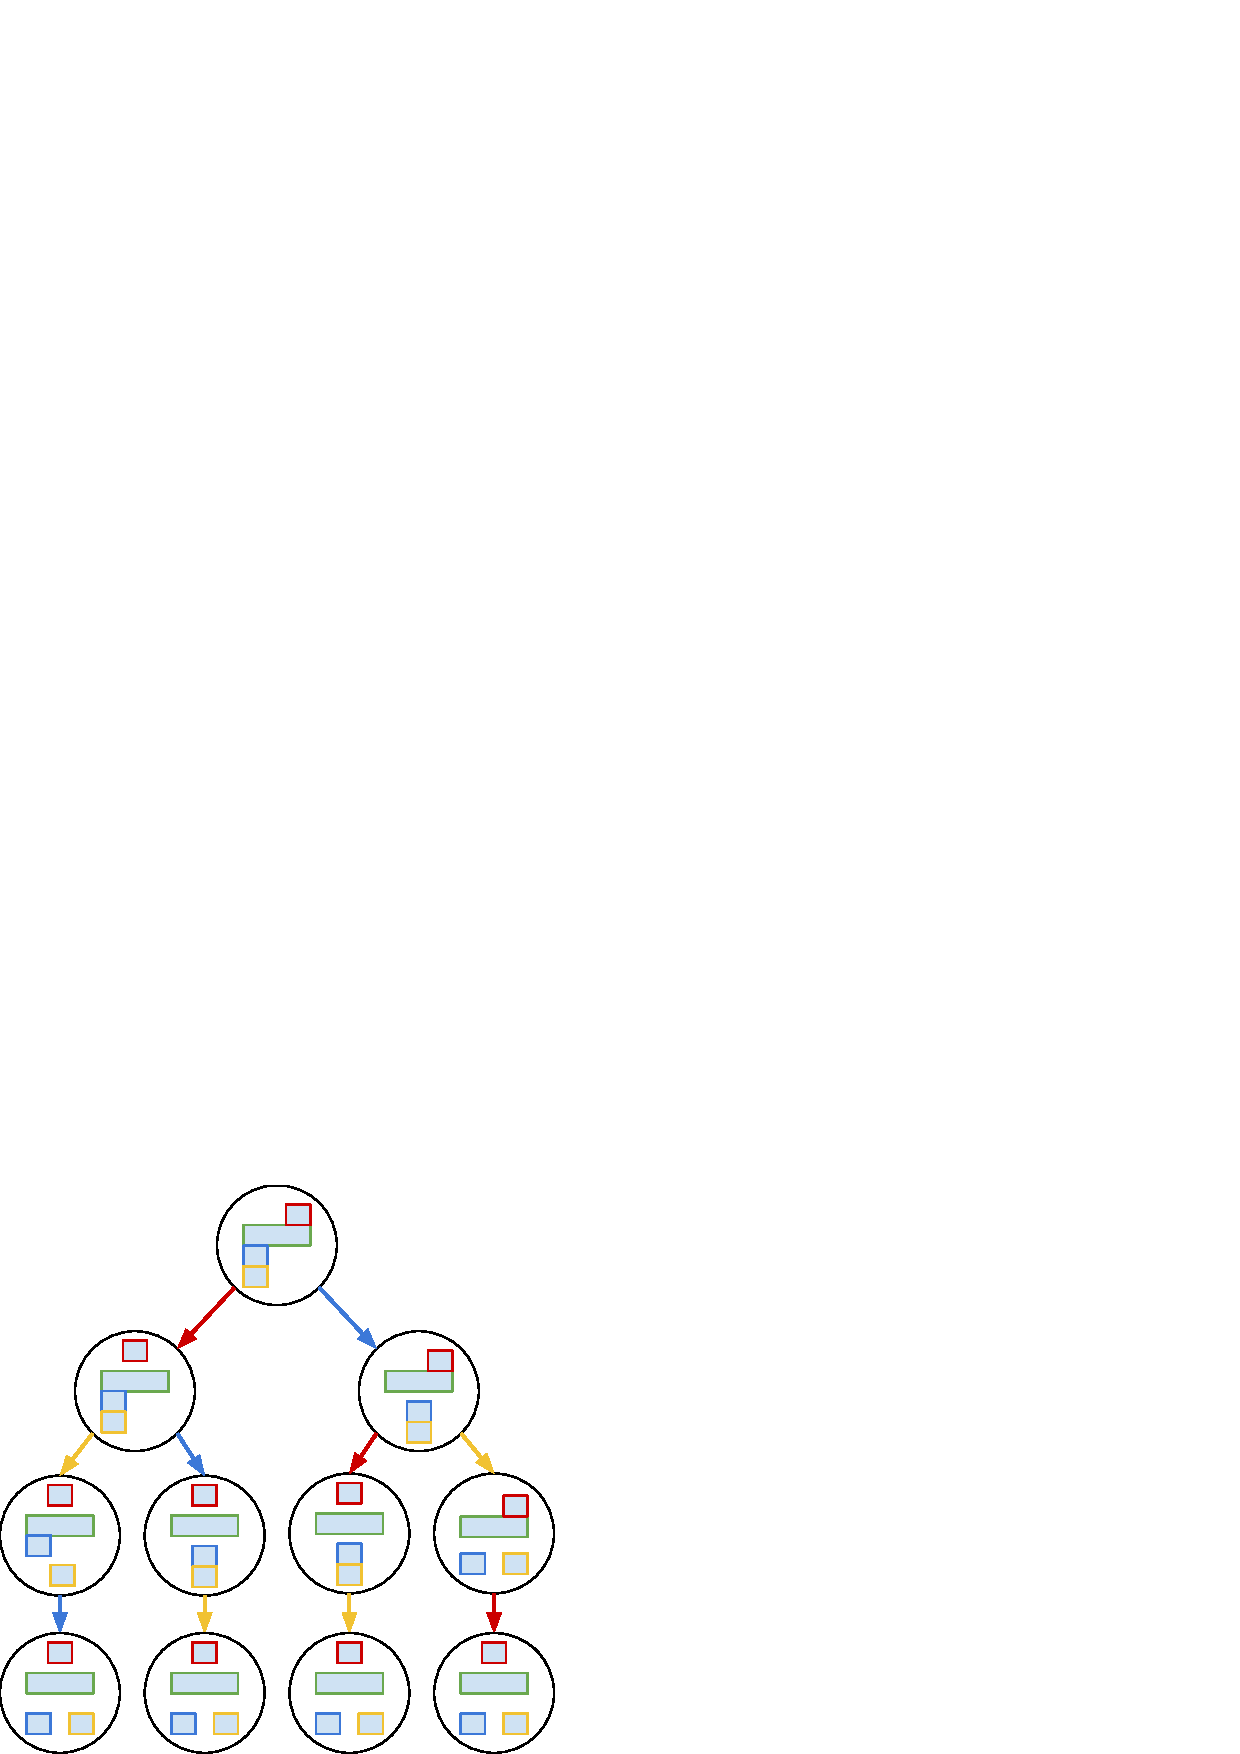
\includegraphics[width=0.2\textwidth]{figs/Subassembly Tree Generation.jpg}
  \caption{The directed tree graph  $\mathbf{H}$ for the disassembly of a 4 Part Structure}\label{fig: treeGen}
\end{figure}

However, with a couple of modifications to this structure, a much smarter result can be established. Firstly, states in the tree $\mathbf{H}$ that are effectively the same can share the same node, and thus reduces the expansion of the tree very nicely. This results in a cleaner structure, as seen in Fig.~\ref{fig: treeGen2}, and also produces only one disassembled endpoint, which allows for the utilization of a lot more traditional graph exploration algorithms.

\begin{figure}[!htb]
\centering
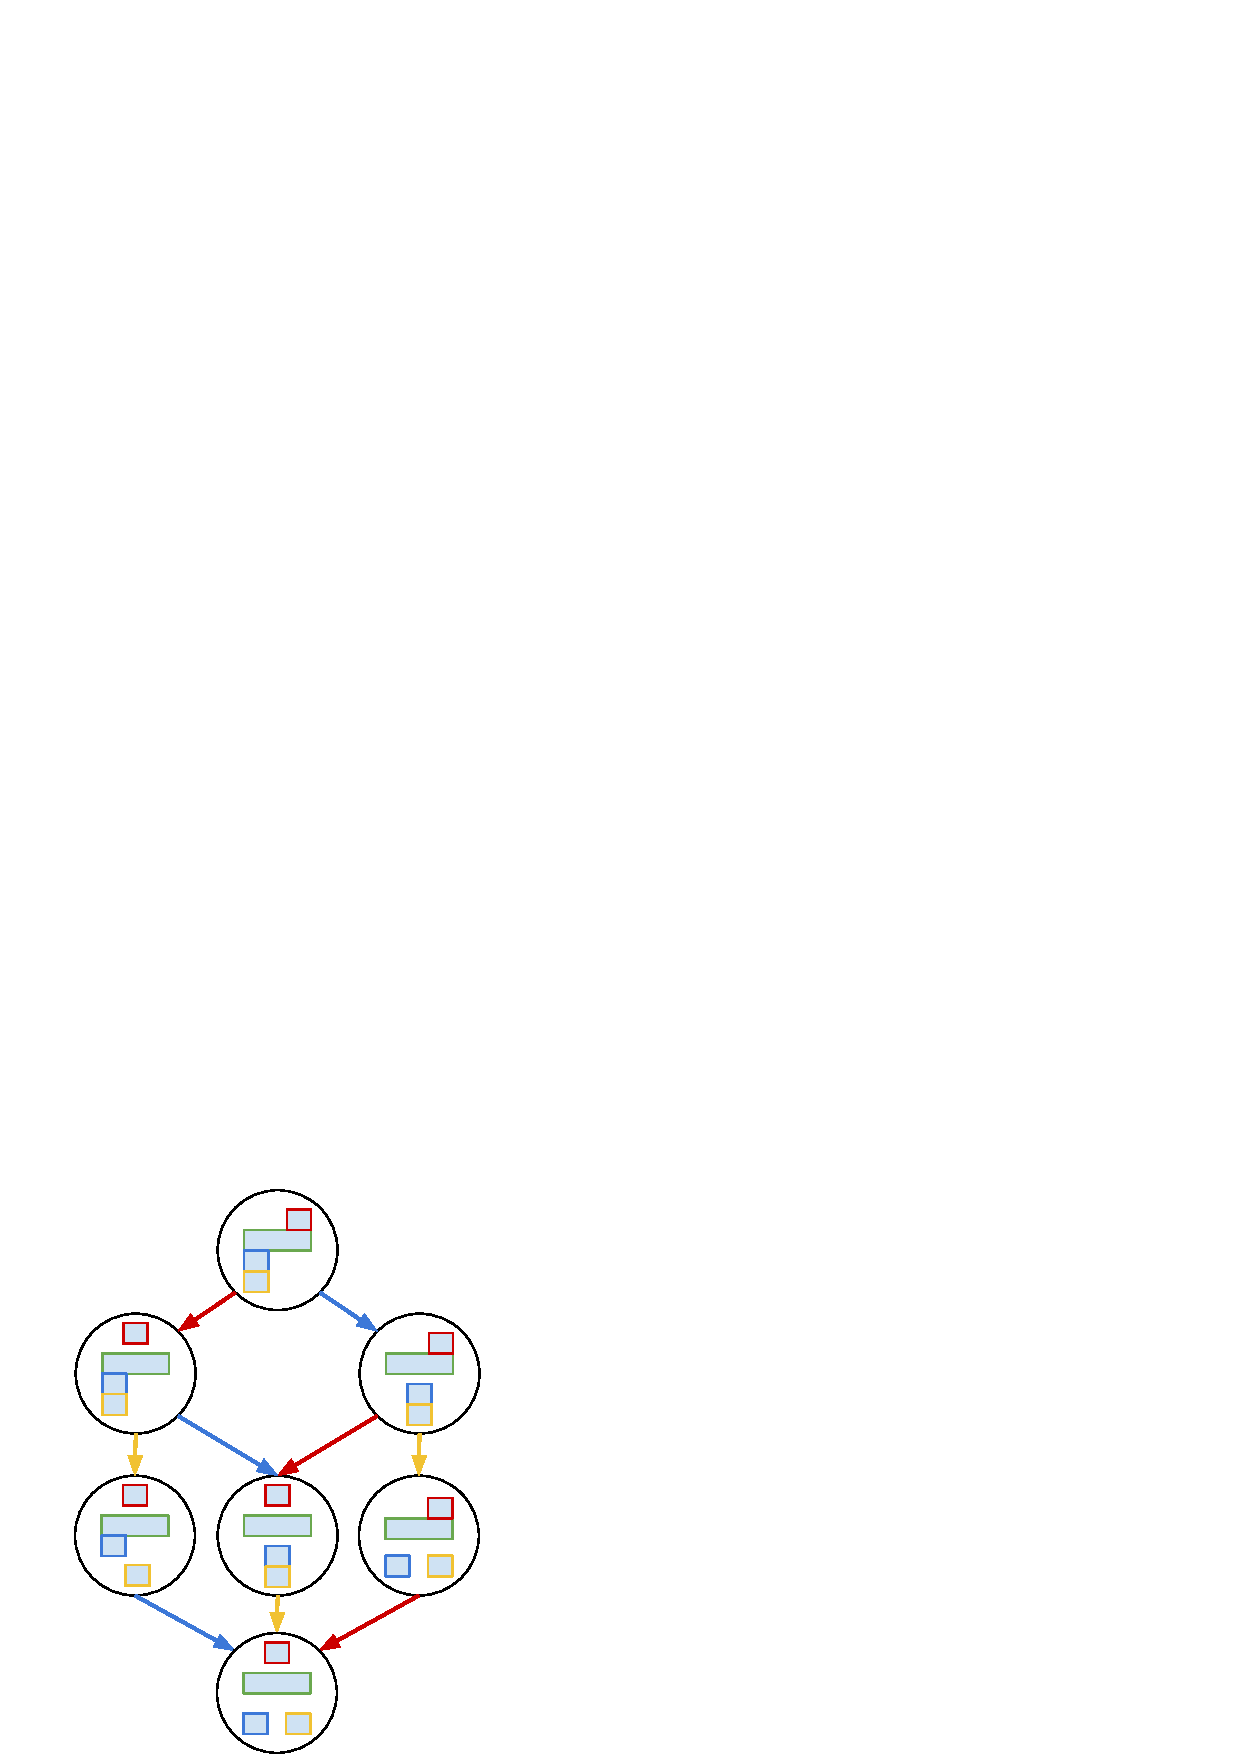
\includegraphics[width=0.2\textwidth]{figs/Consolidated Subassembly Tree Generation.jpg}
  \caption{The Consolidated tree graph  $\mathbf{H}$ for the disassembly of a 4 Part Structure}\label{fig: treeGen2}
\end{figure}

Additionally, if the definition of an \textit{action} is expanded, better results can be ascertained. More precisely, for multi-agent scenarios, the actions can be allowed to include the removal of multiple connections at once, between nodes. Movement of multi-part pieces of the structure can also be codified as an action, in the case of multiple construction zones being available.

\subsection{Constraints Definition}
In consistent vocabulary with the Markov Decision Processes(MDPs) framework, a Probability Transition function $P(s'|s,a), s\in\mathbf{S}, a\in\mathbf{A}$ can be utilized for constraint definitions. For example, if there is some kind of sequential constraint to the assembly (i.e. the center part in a lattice structure must be placed before the parts around it are placed), then this constraint is equivalent to the probability transition between certain state transfers being 0, i.e. impossible. This translates to a particular branch being abandoned on the tree graph $\mathbf{H}$.

As these constraints can utilize information about the intermediate state of the structure, they can be a lot more vague. {\color{red}[PH]}

Additionally, these constraints can greatly reduce the amount of nodes generated in the graph $\mathbf{H}$, thus making the tree generation process shorter and making the graph smaller for later exploration. In this way, the algorithm scales not only well with constraints, but also better with constraints.

\subsection{Exploration Algorithms}
{\color{red}[PH]}
% Cover the usual BFS, DFS, Djikstra's, etc

\subsection{Q-Learning and DQNs}
\color{red} [Transition sentence: however, even these methods fail to produce proper results for very large structures...] \color{black} A DQN is a reinforcement learning algorithm that uses a deep neural network to approximate the Q-function of an agent in a Markov Decision Process (MDP) environment. This deep neural network structure allows the DQN to handle high-dimensional input spaces and in our case, the ability to learn directly from raw state-action-reward data {\color{red}Fix the end of this sentence}.

For the assembly sequencing problem, the DQN algorithm, will utilize the same definition of state and action as above, and to translate this result to the input of a neural network, the following indicator function will be utilized:
\begin{align*}
    \mathcal{I}(E_i) = 
    \begin{cases}
        1 & \text{if Edge } i \text{ is Connected}\\
        0 & \text{if Edge } i \text{ is Disconnected}\\
    \end{cases}
\end{align*}

such that a given state $s$ is indicated via a vector $s \in \mathbf{R}^n$ where $n$ is the number of edges in the completed assembly. The output of this DQN will then be a vector $q \in \mathbf{R}^n$ with $q_i$ indicating an estimate of the Q-value of the given action $i$ (i.e. removal of edge $i$). Observe that as this method returns q-values, any constraints placed on state transitions can still be employed. As such, the DQN follows the neural network architecture laid out in Fig.~\ref{fig: DQN}, and employs the use of an experience replay buffer during training to reduce correlations between consecutive updates of the network. While this method was sufficient for our results, additional modifications can supercharge the DQN algorithm, such as the use of double Q-learning, prioritized experience replay, or dueling network architectures.

\begin{figure}[!htb]
\centering
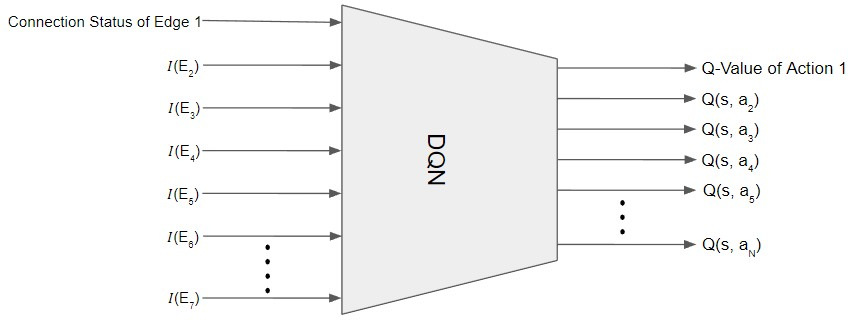
\includegraphics[width=0.5\textwidth]{figs/DQN Architecture.jpg}
  \caption{An overview of the DQN Architecture}\label{fig: DQN}
\end{figure}

{\color{red}[Forgot to mention $\epsilon$-greedy!]}

\section{Experimental Results}
\label{sec:result}
    % Include a table with runtimes and breakdown
	Nam dui ligula, fringilla a, euismod sodales, sollicitudin vel, wisi. Morbi auctor lorem non justo.
	Nam lacus libero, pretium at, lobortis vitae, ultricies et, tellus. Donec aliquet, tortor sed accumsan
	bibendum, erat ligula aliquet magna, vitae ornare odio metus a mi. Morbi ac orci et nisl hendrerit
	mollis. 

	Suspendisse ut massa. Cras nec ante. Pellentesque a nulla. Cum sociis natoque penatibus
	et magnis dis parturient montes, nascetur ridiculus mus. Aliquam tincidunt urna. Nulla ullamcorper
	vestibulum turpis. Pellentesque cursus luctus mauris.
	
	Nulla malesuada porttitor diam. Donec felis erat, congue non, volutpat at, tincidunt tristique, libero.
	Vivamus viverra fermentum felis. Donec nonummy pellentesque ante. Phasellus adipiscing semper 	elit. 
	Proin fermentum massa ac quam. Sed diam turpis, molestie vitae, placerat a, molestie nec, leo.
	Maecenas lacinia. Nam ipsum ligula, eleifend at, accumsan nec, suscipit a, ipsum. Morbi blandit
	ligula feugiat magna. Nunc eleifend consequat lorem. Sed lacinia nulla vitae enim. Pellentesque tin-
	cidunt purus vel magna. Integer non enim. Praesent euismod nunc eu purus. Donec bibendum quam
	in tellus. Nullam cursus pulvinar lectus. Donec et mi. Nam vulputate metus eu enim. Vestibulum
	pellentesque felis eu massa.
	Quisque ullamcorper placerat ipsum. Cras nibh. Morbi vel justo vitae lacus tincidunt ultrices. 
	
	Lorem
	ipsum dolor sit amet, consectetuer adipiscing elit. In hac habitasse platea dictumst. Integer tempus
	convallis augue. Etiam facilisis. Nunc elementum fermentum wisi. Aenean placerat. Ut imperdiet,
	enim sed gravida sollicitudin, felis odio placerat quam, ac pulvinar elit purus eget enim. Nunc vitae
	tortor. Proin tempus nibh sit amet nisl. Vivamus quis tortor vitae risus porta vehicula.

%===============================================================================

\section{Conclusion}
\label{sec:conclusion}

	Nam dui ligula, fringilla a, euismod sodales, sollicitudin vel, wisi. Morbi auctor lorem non justo.
	Nam lacus libero, pretium at, lobortis vitae, ultricies et, tellus. Donec aliquet, tortor sed accumsan
	bibendum, erat ligula aliquet magna, vitae ornare odio metus a mi. Morbi ac orci et nisl hendrerit
	mollis. Suspendisse ut massa. Cras nec ante. Pellentesque a nulla. Cum sociis natoque penatibus
	et magnis dis parturient montes, nascetur ridiculus mus. Aliquam tincidunt urna. Nulla ullamcorper
	vestibulum turpis. Pellentesque cursus luctus mauris.
	Nulla malesuada porttitor diam. Donec felis erat, congue non, volutpat at, tincidunt tristique, libero.
	Vivamus viverra fermentum felis. Donec nonummy pellentesque ante. Phasellus adipiscing semper
	elit. Proin fermentum massa ac quam. Sed diam turpis, molestie vitae, placerat a, molestie nec, leo.
	Maecenas lacinia. Nam ipsum ligula, eleifend at, accumsan nec, suscipit a, ipsum. Morbi blandit
	ligula feugiat magna. Nunc eleifend consequat lorem. Sed lacinia nulla vitae enim. Pellentesque tin-
	cidunt purus vel magna. Integer non enim. Praesent euismod nunc eu purus. Donec bibendum quam
	in tellus. Nullam cursus pulvinar lectus. Donec et mi. Nam vulputate metus eu enim. Vestibulum
	pellentesque felis eu massa.
	Quisque ullamcorper placerat ipsum. Cras nibh. Morbi vel justo vitae lacus tincidunt ultrices. Lorem
	ipsum dolor sit amet, consectetuer adipiscing elit. In hac habitasse platea dictumst. Integer tempus
	convallis augue. Etiam facilisis. Nunc elementum fermentum wisi. Aenean placerat. Ut imperdiet,
	enim sed gravida sollicitudin, felis odio placerat quam, ac pulvinar elit purus eget enim. Nunc vitae
	tortor. Proin tempus nibh sit amet nisl. Vivamus quis tortor vitae risus porta vehicula.

%===============================================================================

\clearpage
% The acknowledgments are automatically included only in the final and preprint versions of the paper.
\acknowledgments{If a paper is accepted, the final camera-ready version will (and probably should) include acknowledgments. All acknowledgments go at the end of the paper, including thanks to reviewers who gave useful comments, to colleagues who contributed to the ideas, and to funding agencies and corporate sponsors that provided financial support.}

%===============================================================================

% no \bibliographystyle is required, since the corl style is automatically used.
\bibliography{example}  % .bib

\end{document}
